\documentclass[border=5pt,convert]{standalone}
%\documentclass[12pt, landscape]{article}

\setlength{\textwidth}{49cm}

\usepackage{tikz}
\usetikzlibrary{calc,intersections,angles,quotes}
\usepackage{amssymb}

\begin{document}
\vspace*{3cm}
\hspace*{-1cm}



%\begin{center}
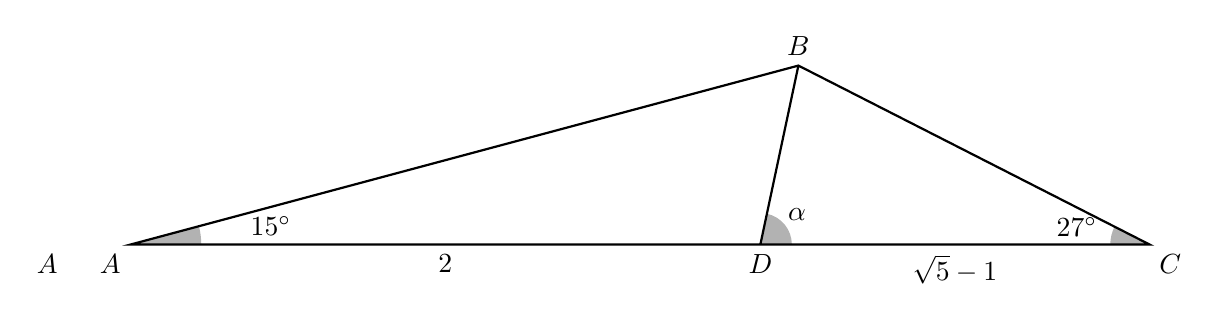
\begin{tikzpicture}[scale=4]
    \coordinate[label=below left:$A$] (A) at (0,0);
    \coordinate[label=below left:$A$] (O) at (-0.2,0);
    \coordinate[label=below right:$C$] (C) at ($(A)+(0:{sqrt(5)+1})$);
    \path[name path=lineAA] (A) -- ($(A)+(15:{2.4})$);
    \path[name path=lineCC] (C) -- ($(C)+(153:{1.5})$);
    \path[name intersections={of = lineAA and lineCC}]; 
    \coordinate[label=above:$B$] (B) at (intersection-1);
    \coordinate[label=below:$D$] (D) at ($(A)+(0:{2})$);
    
    \draw pic["$15^\circ$", fill=gray!60, -, angle eccentricity=2, angle radius=0.9cm] {angle=C--A--B};
    \draw pic["$27^\circ$", fill=gray!60, -, angle eccentricity=1.9, angle radius=0.5cm] {angle=B--C--A};
    \draw pic["$\alpha$", fill=gray!60, -, angle eccentricity=1.5, angle radius=0.4cm] {angle=C--D--B};
    
    \draw[thick]
    	(A) -- node[below] {$2$}
    	(D) -- node[below] {$\sqrt{5}-1$}
    	(C) -- (B) -- cycle
    	(D) -- (B);
    	
    
\end{tikzpicture}
%\end{center}

\end{document}
